\section{DESCRIPCIÓN DE LOS DATOS}

Como se ha comentado anteriormente, la búsqueda por mejorar las condiciones animales en los procesos de crianza ha fomentado la investigación en 
diferentes marcadores biológicos.

El \acrfull{pran}\cite{ObservatorioUPM}, perteneciente a la \acrfull{ETSIAAB}, realiza investigaciones en estas líneas, siendo una principal el bienestar animal en peces, 
usando experimentos como el \textit{NetTest}.

A partir de estas labores anteriores de investigación, se han podido obtener materiales para este trabajo, siendo principalmente videos del experimento junto a sus etiquetas. Para obtener 
estos datos, en sucesivos trabajos del \acrshort{pran} se ha utilizado la herramienta \textit{BORIS}\cite{friardBORISFreeVersatile2016}, que ha permitido anotar diferentes momentos en los que 
ha sucedido un movimiento.

Es importante saber que este etiquetado manual no siempre se ha llevado a cabo por la misma persona, y por lo tanto, hay un factor de subjetividad que añade error humano a la medición de los 
movimientos de los peces.

\subsection{Conjunto de datos disponibles: videos}

Los videos se pueden separar en 2 subconjuntos dependiendo del momento en el que se realizó la grabación, lo cual se ve reflejado en la calidad de la grabación.

\subsubsection{Videos antiguos}

Se tratan de videos en formato \texttt{16:9}, con resolución \texttt{1920x1080}, con la cámara posicionada fija verticalmente encima de una mesa donde se lleva a cabo el experimento. Esto se puede ver 
en la \autoref{fig:ExperimentoAntiguo}. En este caso, el experimento se lleva a cabo con redes negras, lo cual puede ser problemático teniendo en cuenta que los peces tienen 
tonalidades similares al marrón y grises.

\begin{figure}[h]
    \centering
    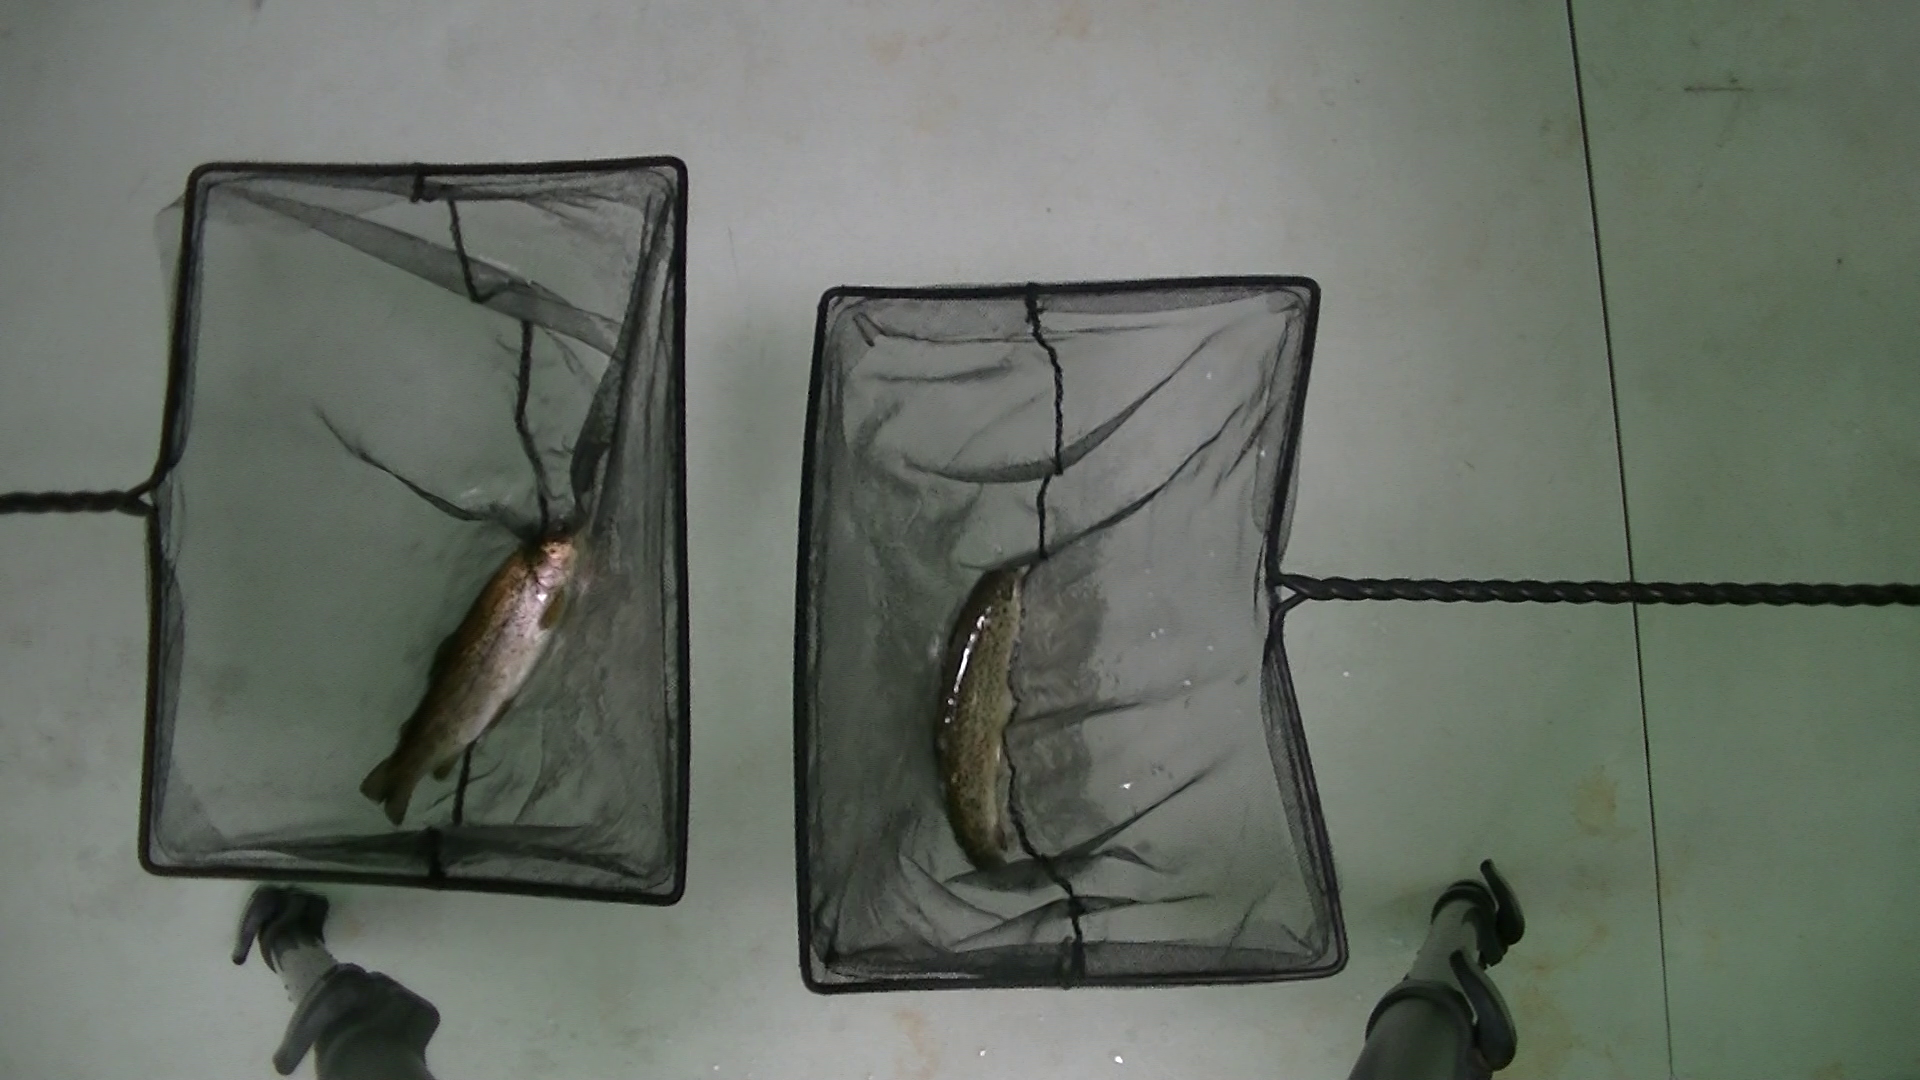
\includegraphics[width=0.70\textwidth]{images/3/ExperimentoAntiguo.png}
    \caption{Aspecto de los videos más antiguos}
    \label{fig:ExperimentoAntiguo}
\end{figure}

Las especificaciones de la cámara en el momento de grabación son desconocidas, pero a través de los detalles de los archivos se observa que son archivos con extensión 
\textit{\acrfull{mts}}, grabados a 25 \acrshort{fps} y con un bitrate (tasa de datos por segundo) de \texttt{16.96 Mbps}.

En estos videos, se realizan el experimento 5 veces con 2 peces a la vez para maximizar el tiempo. Por lo tanto, puede ser necesario segmentarlo manualmente.

Como último punto importante, en estos videos se puede observar que se realiza la variación del \textit{NetTest} que dura 1 minuto aproximadamente.

\subsubsection{Videos nuevos}

Los videos mantienen las características de formato en \texttt{16:9}, con resolución \texttt{1920x1080} y cámara apuntando verticalmente a la mesa del experimento 
(\autoref{fig:ExperimentoNuevo}), sin embargo, podemos ver que se ha pasado a usar una red verde que aporta cierto contraste respecto al cuerpo del pez. Aparte de esto, 
el marco de la red también ha cambiado y tiene un color plateado.

\begin{figure}[h]
    \centering
    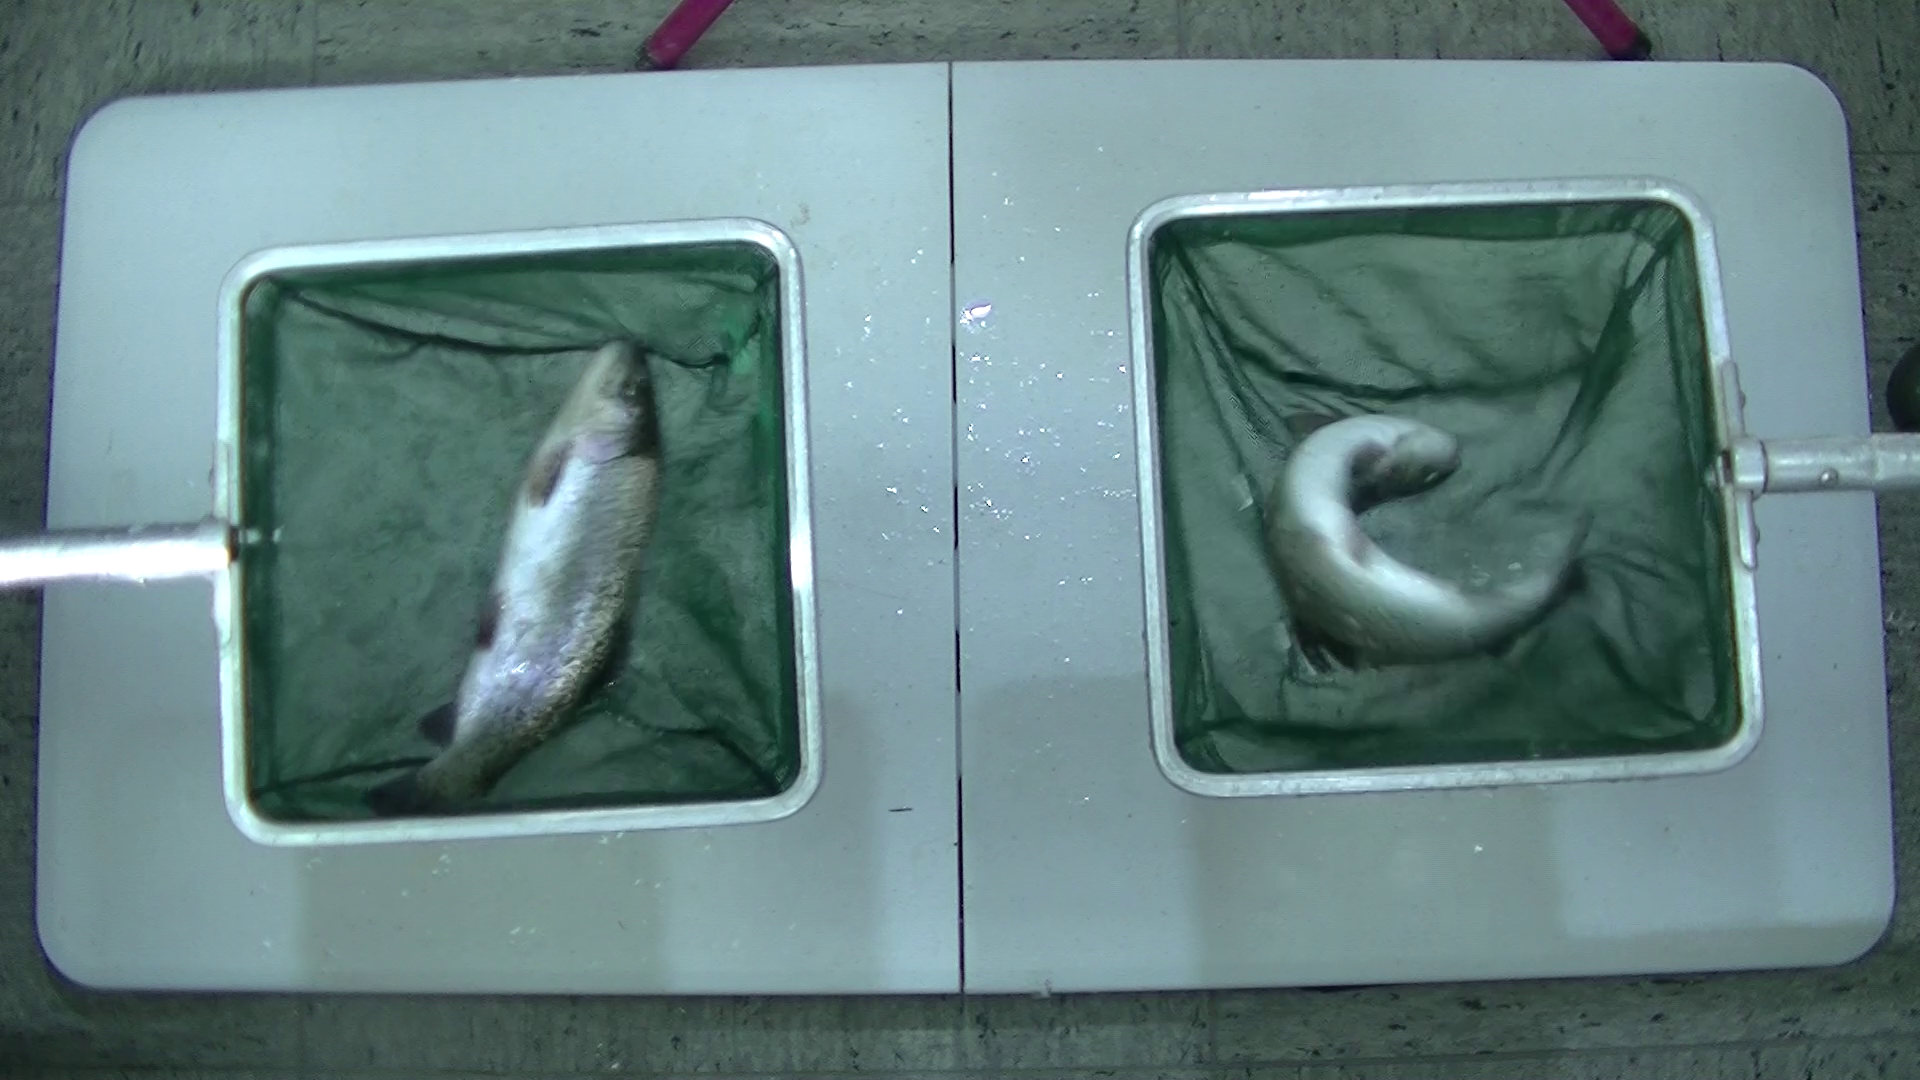
\includegraphics[width=0.75\textwidth]{images/3/ExperimentoNuevo.png}
    \caption{Aspecto de los videos nuevos}
    \label{fig:ExperimentoNuevo}
\end{figure}

Las especificaciones de la cámara para estos videos siguen siendo desconocidas, pero se puede asumir que los parámetros han cambiado por el aumento de la luminosidad de la imagen.
Además, se ha movido un poco la colocación de la mesa y la línea negra queda justo en el medio entre las dos truchas con las que se realiza el experimento.

Respecto a datos técnicos del video, el contenedor ha cambiado a \textit{\acrfull{mov}}, se mantienen los 25 \acrshort{fps} y el bitrate aumenta hasta los \texttt{21 Mbps}.

Los videos obtenidos en este caso también contienen videos de experimentos en grupo, es decir, varios experimentos a varias parejas de truchas. Sin embargo, a diferencia de los videos antiguos, 
en este caso los experimentos \textit{NetTest} duran 15 segundos aproximadamente.

\subsection{Conjunto de datos disponibles: etiquetas}

En este caso,




